% classes
\documentclass{article}

% packages
\usepackage{graphicx}
\usepackage{fancyhdr} % Required for custom headers
\usepackage{lastpage} % Required to determine the last page for the footer
\usepackage{extramarks} % Required for headers and footers
\usepackage{courier} % Required for the courier font

\usepackage{color}
\usepackage{enumitem}

\usepackage{hyperref}


% page layout

\topmargin=-0.45in
\evensidemargin=0in
\oddsidemargin=0in

\textwidth=6.5in
\textheight=9.0in

\headsep=0.25in

\linespread{1.1} % Line spacing
 
\pagestyle{fancy}

% headers and footers

\fancyhf{}

\lhead{INTR 100 Breaking Intuition}

\rhead{
\includegraphics[width=0.045\textwidth]{wmlogo.jpg}}



% document body

\begin{document}

\vspace*{.01mm}

\begin{center}

\Large{\textcolor{blue}{\textbf{Lab 2.}  Introduction to Visualising Spatial Data with R}}

\vspace{4mm}

\textit{Due by noon on Friday, September 11th}\\

\end{center}

\begin{figure}[h!]
\begin{center}
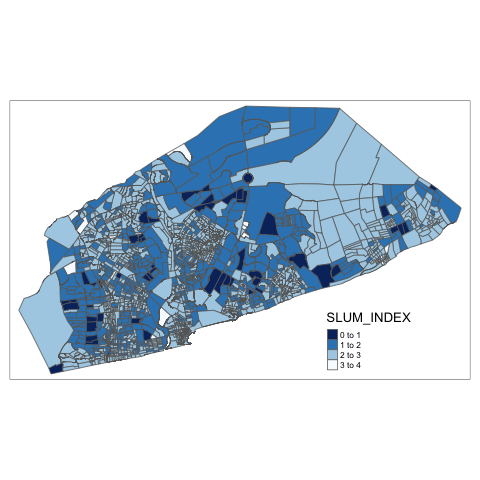
\includegraphics[width=0.9\textwidth]{accra.png}

\end{center}
\end{figure}

\setlength{\parindent}{0cm}

\large{\textit{"Everything is related to everything else, but near things are more related than distant things."}
\begin{flushright}
Tobler, 1970
\end{flushright}
}


\newpage

% Enumerate the Laboratory Objectives

\large{\textbf{Laboratory in Brief:}}

\vspace{4mm}

\setlength{\leftskip}{1cm}

\setlength{\parindent}{0cm}

The purpose of this laboratory is to introduce students to working with spatial data by ...

\vspace{4mm}

\setlength{\leftskip}{0cm}

\large{\textbf{Specific Objectives:}}

\begin{enumerate}[leftmargin=15mm]

\item To install use the packages ...

\item To use the functions ...

\item To do this ...

\end{enumerate}

% Enumerate the Laboratory Objectives

\large{\textbf{Software and Resources you will need or will be helpful:}}

\begin{enumerate}[leftmargin=15mm]

\item The R Project for Statistical Computing otherwise known simply as R.  The R framework can be downloaded from \\ 
\url{https://www.r-project.org/}

\item item 2 ...

\item item 3 ...

\end{enumerate}


\large{\textbf{Step by Step Instructions:}}

\begin{enumerate}[leftmargin=15mm]

\item Create a Map using Leaflet

\item Create a Map using GGMap

\item Create a Map using TMAP

\item Do some spatial descriptive statistics using TMAP \& GGMAP

\end{enumerate}


\textbf{Grading}

\vspace{4mm}

\setlength{\leftskip}{1cm}

\setlength{\parindent}{0cm}

You will be graded like so ...   \\

Your lab report should include the following elements.

\begin{enumerate}[leftmargin=15mm]

\item all three maps, including description an analysis of each one

\item integrated into your report, a description of the code you used, in a manner that demonstrates your knowledge of how the code functioned and operated

\item an analysis of how increased disaggregation effects the statistical description of spatial data

\end{enumerate}

The highest grades will be reserved for work that not only spatially describes your chosen area in a statistically rigorous manner, but also uses quantitative analysis to suggest and support inferential conclusions. \\

\vspace{7mm}

\setlength{\leftskip}{0cm}

%----------------------------------------------------------------------------------------

\end{document}